\documentclass[letterpaper, titlepage, 11pt]{article}

\usepackage{hyperref}
\usepackage[toc,page]{appendix}
\usepackage{graphicx}
\usepackage{caption}
\usepackage{subcaption}
\usepackage{amsmath}
\usepackage{listings}
\usepackage{color}
\definecolor{mygreen}{RGB}{28,172,0} % color values Red, Green, Blue
\definecolor{mylilas}{RGB}{170,55,241}
\lstset{language=Matlab,%
    basicstyle=\footnotesize,
    breaklines=true,%
    morekeywords={matlab2tikz},
    keywordstyle=\color{blue},%
    morekeywords=[2]{1}, keywordstyle=[2]{\color{black}},
    identifierstyle=\color{black},%
    stringstyle=\color{mylilas},
    commentstyle=\color{mygreen},%
    showstringspaces=false,%without this there will be a symbol in the places where there is a space
    numbers=left,%
    numberstyle={\tiny \color{black}},% size of the numbers
    numbersep=9pt, % this defines how far the numbers are from the text
    emph=[1]{for,end,break},emphstyle=[1]\color{red}, %some words to emphasise
    %emph=[2]{word1,word2}, emphstyle=[2]{style},
}
\title{Implementation of a Real-Time Spectrum Analyzer Synthesized on FPGA}
\author{David Lavoie-Boutin, 260583602}
\date{\today}


\begin{document}

\maketitle
\begin{abstract}\
As a final project for the Signal Processing Hardware course (ECSE 436), I was tasked with designing, implementing and deploying a Real-Time spectrum analyzer. This project included the custom implementation of the FFT algorithm in Matlab, porting that algorithm to HDL code that would be synthesized for an FPGA, the acquisition of audio samples and display of the FFT results on the same FPGA. To achieve this goal, I implemented the common Cooley–Tukey algorithm for computing the FFT. I used Matlab and Simulink to generate the HDL code for the FFT algorithm based on the Simulink testbench created. I created the control logic modules to prepare the samples for the FFT and parse its output for the display module, which displays the magnitude of each FFT coefficient output.
\end{abstract}

\tableofcontents
\clearpage

\section{Introduction \& Background}
The FFT algorithm is often considered as one of the algorithms that revolutionized the world, some even say, "the most important of our lifetime"~\cite{important}. Its applications are virtually endless and range from simple voice analysis to radar to every form of communication we know of. For this project, I had to create an audio spectrum analyzer that would employ the FFT to decompose the signal in its frequency components and display the magnitude of each component on a computer monitor. \\
\\
In the end, this entire system was to run on an Altera DE-II development board which integrates the Cyclone II FGPA with a bunch of other dedicated controllers, including RAM, ADCs, USB, etc. First, I developed my custom implementation of the Cooley–Tukey FFT algorithm in Matlab. Then I created a Simulink testbench using Matlab's FFT function, optimized for HDL synthesis and used Matlab to generate the HDL code for the FFT.\\
\\
I integrated the generated code the to rest of the FPGA project and linked it with some control logic to the acquisition system. The output of the FFT are then buffered until all the data is available and displayed on a VGA monitor. For this, I designed a simple module that plots an array of data in a bar chart.

\section{Matlab Algorithm}
The Matlab algorithm I implemented for the computation of the FFT follows very closely the Cooley–Tukey algorithm described on Wikipedia~\cite{wiki_cooley} and further developed in a paper by Stefan Worner~\cite{fft_it}. My first implementation followed the recursive strategy and the second uses the iterative strategy:
\lstinputlisting[language=Matlab, caption="Recursive FFT implementation"]{../myFFT.m}
\lstinputlisting[language=Matlab, caption="Iterative FFT implementation"]{../fft_it.m}

After implementing my own version of FFT, I considered using Matlab to generate synthesizable HDL code. Using Simulink and the DSP toolbox, I used the HDL optimized FFT function in the example diagram shipped with Matlab and adapted it to my input specifications. The schematic is illustrated in figure~\ref{fig:simulink}.
\begin{figure}[!htb]
  \centering
  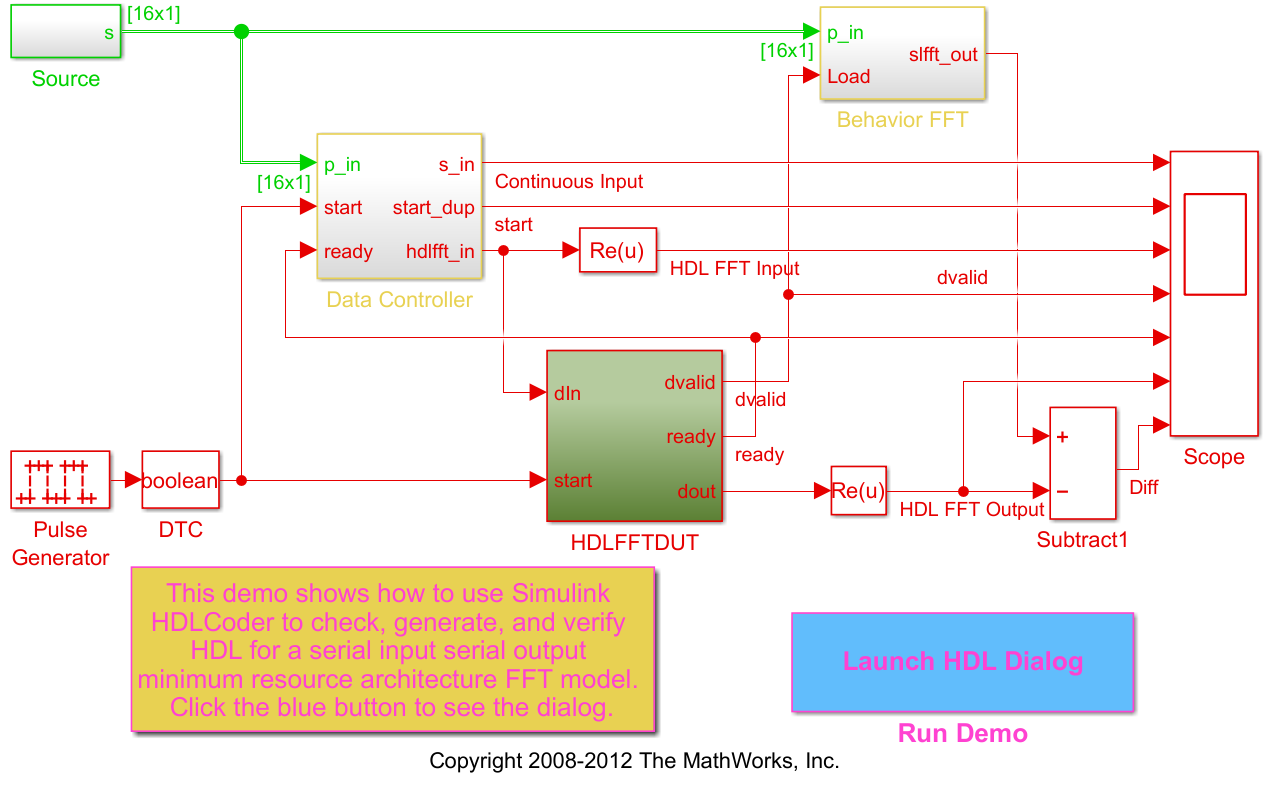
\includegraphics[width=0.8\textwidth]{sim2.PNG}
  \caption{Simulink schematic of a HDL optimized FFT}
  \label{fig:simulink}
\end{figure}

Running the simulation compares the output of the built-in FFT function to the HDL optimized FFT function and we can see that they do not match. This is due to the optimization strategy of the HDL block where the $e^x$ function is replaced with a lookup table which is not as precise as the native function. With this schematic established, I was able to use the HD Coder function in Matlab to generate the VHDL code for the FFT component.

\section{Display on the FPGA}
Before implementing the full processing to display pipeline, I created and tested the display module on its own using the infrastructure provided in Lab 3. For this purpose, I designed a modular block that displays an array of values as a bar chart. There are several interesting points I want to outline in the implementation of this block.

\subsection{Package Definitions}
In order to maximize modularity of the code developed, I choose to define custom types and package constants to parameters that would be used in different modules and that were susceptible to change frequently in the life of the project. These include a specific data type to pass values to display as an array, the number of data samples and the number of bits used to represent those samples.

\lstinputlisting[language=VHDL, firstline=5, lastline=10]{../VideoLab/graph_display.vhd}

\subsection{Modular Bar Chart}
Another interesting design point in this graphing module is the use of compilation time resolution of different parameters such as the number of bars and the width of each bars. This is done using simple arithmetic, but makes the design very modular simply using the constants described earlier.

\lstinputlisting[language=VHDL, firstline=47, lastline=49]{../VideoLab/graph_display.vhd}

\subsection{Array Input}
The last point I want to mention is the use of custom types to pass and manipulate the set of data to graph. The use of the array type make is easy to address the data elements using simple indexes and allows us to iterate on the data using a ``for loop'' construct in VHDL.
\begin{lstlisting}[language=VHDL]
for j in 0 to NUMBER_OF_SAMPLES-1 loop
    temp := pad & switch(j*switch_range_width+switch_range_width-1 downto j*switch_range_width);
    data(j) <= temp(SAMPLES_DATA_LENGTH -5 downto 0) & "0000";  -- convert range of switches to data element
end loop;
\end{lstlisting}

\subsection{Switch to Test}
In order to test this design, I used the switches on the board to emulate data and confirm the good behavior of the module. First I created a module that converts the vector of switch values to the data array type I defined.

\lstinputlisting[language=VHDL, firstline=7]{../VideoLab/switch_to_array.vhd}

I then used Modelsim to simulate this module and confirm its good behavior which yielded figure~\ref{fig:switch_sim}. In the figure we can see that each sample is represented by a group of 4 switches and that switches 17 and 18 are not mapped to any sample as 18 is not divisible by 4.

\begin{figure}[!htb]
  \centering
  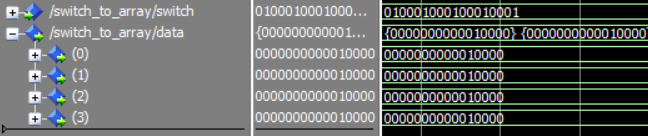
\includegraphics[width=0.8\textwidth]{switch_sim.PNG}
  \caption{Modelsim simulation of the switch to array module}
  \label{fig:switch_sim}
\end{figure}

\section{FFT on FPGA}

After implementing and testing the graphing module, I used the infrastructure provided for lab 2 and modified it with the modules I needed to run the FFT on the audio samples. For this I created the block diagram shown in figure~\ref{fig:block_filter}

\begin{figure}[!htb]
  \centering
  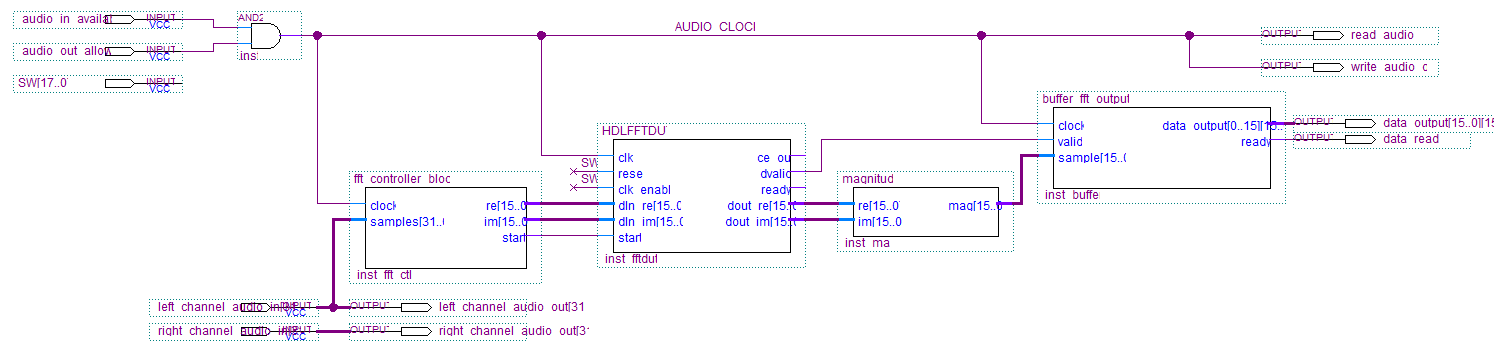
\includegraphics[width=\textwidth]{full_filter.PNG}
  \caption{FFT integration in the audio processing unit}
  \label{fig:block_filter}
\end{figure}

This block diagram show several additional modules. The first block is the data controller. This block simply casts the 32 bit audio sample to a 16 bits representation that the FFT block will use. It also drives the start signal which indicates a new set of inputs for the FFT computation. The data is then passed to the FFT block.

\lstinputlisting[language=VHDL, firstline=6]{../VideoLab/fft_controller_block.vhd}

After the FFT, we compute the magnitude of the coefficients using the traditional geometric norm. This poses the challenge of requiring us to compute the square root of the numbers which is not that trivial. For this task, I used an implementation of the Non-Restoring Square Root Algorithm~\cite{sqrt}.

\lstinputlisting[language=VHDL, firstline=5, caption="Square-Root function"]{../VideoLab/sqrt.vhd}
\lstinputlisting[language=VHDL, firstline=7, caption="Magnitude module"]{../VideoLab/magnitude.vhd}

The last step before displaying the data is to buffer a set of outputs since the FFT outputs the coefficients in series and we want to display all the data at once. For this purpose I implemented a simple buffer module that build an array with the samples and published it once it is filled.

\lstinputlisting[language=VHDL, firstline=7, caption="Buffer module for the FFT output"]{../VideoLab/buffer_fft_output.vhd}

And in order to test the proper behavior of this module, I also created a Modelsim testbench and simulated its behavior. In the simulation results in figure~\ref{fig:buff_sim}, notice how each cell is loaded sequentially and how the ``valid'' signal is set once all the cells are loaded.

\lstinputlisting[caption="Buffer module testbench"]{../VideoLab/buffer_testbench.tcl}

\begin{figure}[!htb]
  \centering
  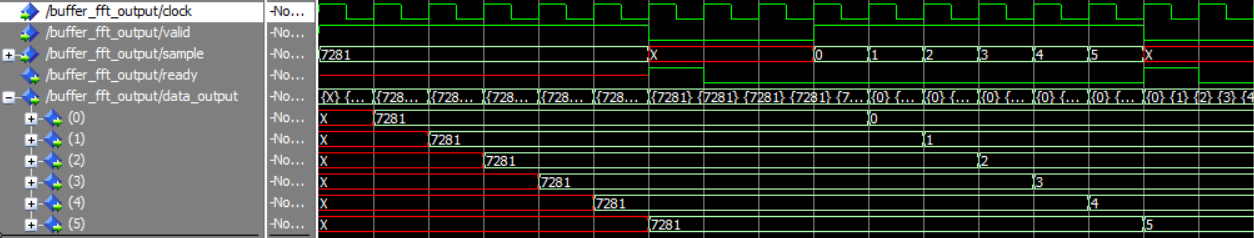
\includegraphics[width=\textwidth]{buffer_sim.PNG}
  \caption{Simulation results for the buffer module}
  \label{fig:buff_sim}
\end{figure}

\section{Conclusion}
For this final project, I designed, implemented, integrated and tested a real-time spectrum analyzer which uses the FFT to decompose a signal in its frequency components which are then plotted on a computer monitor. This implementation was synthesized from Verilog and VHDL code and loaded on a Cyclone II FPGA development board.\\
\\
Preliminary steps in the project included a Matlab and Simulink implementation and simulation of the FFT algorithm, generation of HDL code for the FFT using Matlab, Modelsim simulations of different HDL modules and finally a full deployment and test of the processing pipeline.\\
\\
During the tests with the FPGA, the data observed on the screen was very noisy. I must point out that signal acquired by the FPGA itself was very noisy to begin with so many parasitic frequency components are expected on the output and this is what I observed. When sitting idle, the bars shown on screen oscillated very much very fast, to the point where many samples aliased together and gave the impression the full bars were displayed.\\
\\
When playing a tone, this parasitic noise behavior was still observed, but some bars clearly had more consistent values and we could see a clear value for that bar. Additionally, the position of that bar on the frequency scale matched the frequency of the tone, which leads me to believe this implementation is generally functional. With extra noise filtering efforts, I believe this project to turn to a fully functional analyzer.


\section{References}
\bibliography{sources}
\bibliographystyle{plain}
\end{document}